
%Chapter 2

\renewcommand{\thechapter}{2}

\chapter{The LUX Detector}
\label{Ch:2}

\section{Introduction}

The LUX experiment is located 4850 ft underground (4300 m w.e.) at the Sanford Underground Research Facility in Lead, South Dakota. After running for 85.3 live days in 2013, LUX has set the most sensitive limit for a spin-independent WIMP scattering cross section \cite{LUX_PRL} and is expected to achieve five times the sensitivity after a 300 day run ending in 2015. 

Nobel elements are promising candidates for WIMP detection. They are easy to purify and are transparent to their own scintillation light. Xenon is especially favorable due to its  large atomic mass (131.3 amu) and high liquid phase density ($\rm \sim$2.9 kg/l) which provides both an excellent target for coherent WIMP scattering while simultaneously providing excellent stopping power from external radioactivity. Xenon is also free of any long lived radioactive isotopes which contribute backgrounds for the WIMP search. There are well established techniques to remove and monitor the residual, troublesome radio isotopes of $\rm ^{39}Ar$ and $\rm^{85}Kr$ found in the atmosphere from which the xenon is distilled \cite{Aprile_LXe_overview} \cite{Kr_ppt_Dobi} \cite{lux_kr_removal} \cite{xmass_kr_removal}.
 
WIMPs, being weakly interacting and non-relativistic, primarily interact with the xenon target nuclei producing nuclear recoil (NR) events, whereas typical backgrounds in the detector, gammas and betas, interact with the atomic electrons producing electronic recoils (ER). In liquid xenon ER events can be further discriminated from NR events a factor of 100 or more by measuring the charge to light ratio of the interaction, as explained in section \ref{sec:BG_Rejection}.


\section{The LUX TPC}

 \begin{figure}[h!]\centering
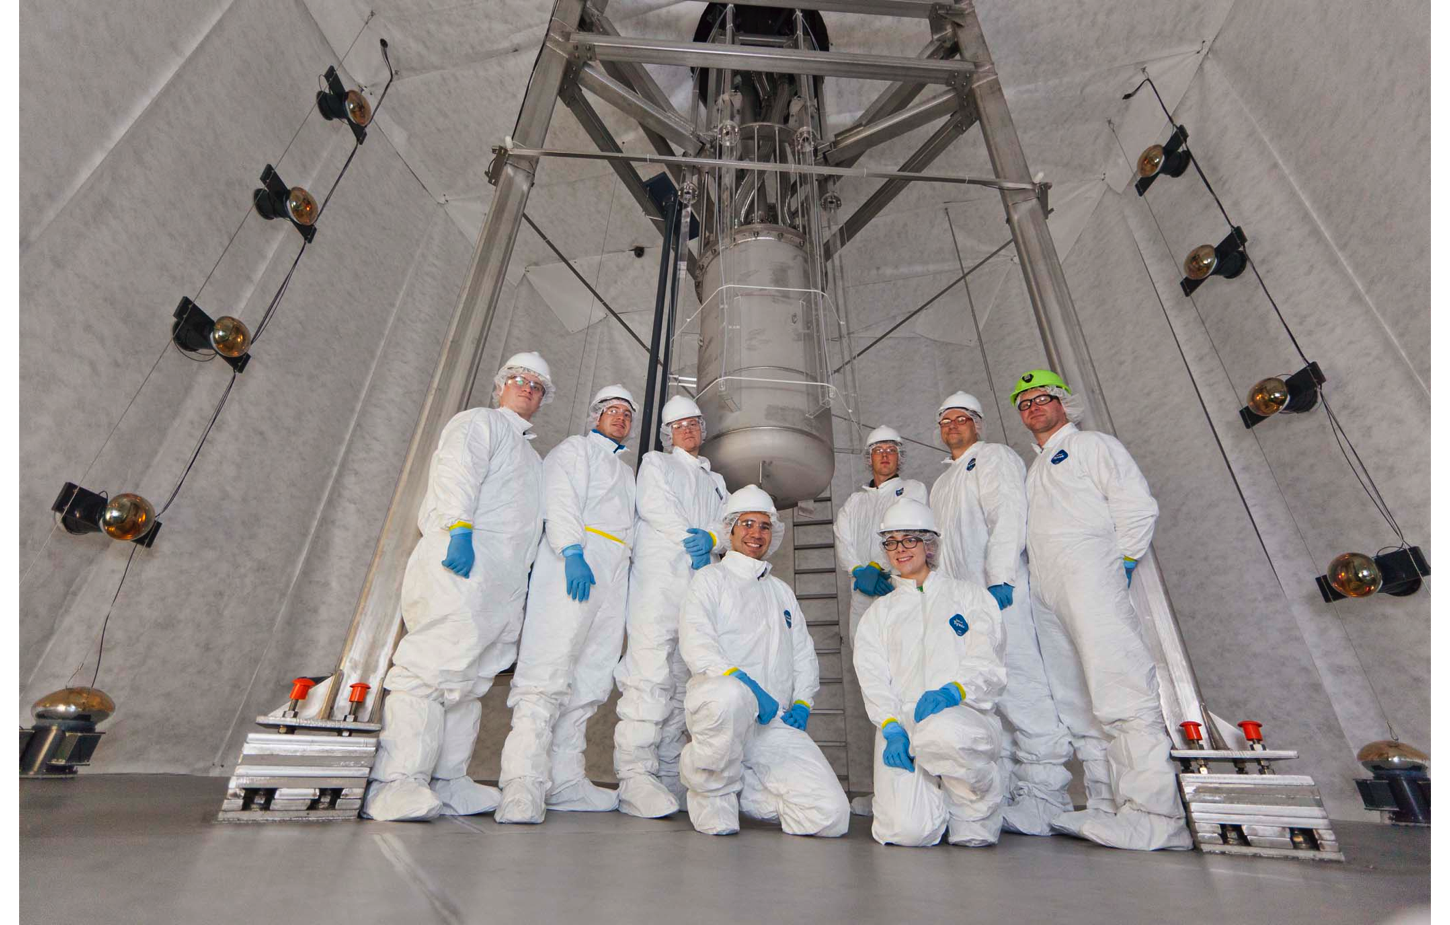
\includegraphics[scale=0.5]{Chapter_LUX_Det/LUX_Real.png}
\caption{Photo of the outer vessel of the LUX detector from inside the water tank.}
\label{fig:LUX_Real}
\end{figure}

%\begin{figure}[h!]\centering
%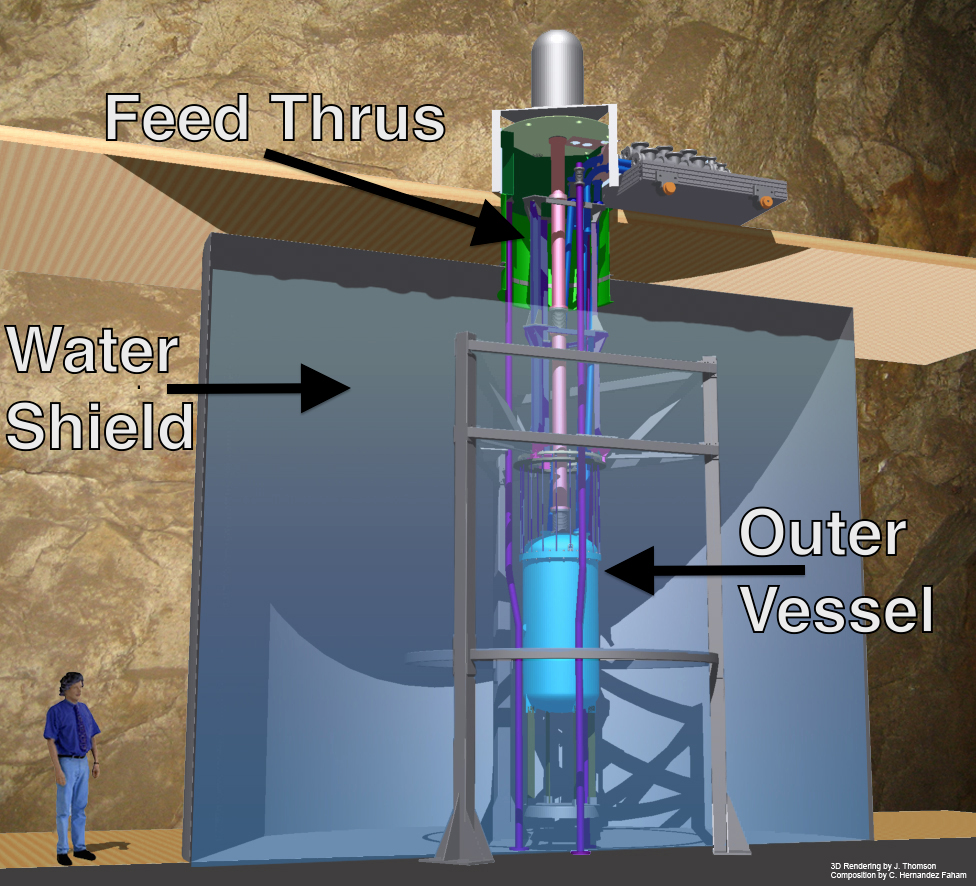
\includegraphics[scale=0.4]{Chapter_LUX_Det/Davis_3D_tank_text.jpg}
%\caption{Schematic of the LUX detector and the surrounding water tank.}
%\label{fig:LUX_Davis}
%\end{figure}

 \begin{figure}[h!]\centering
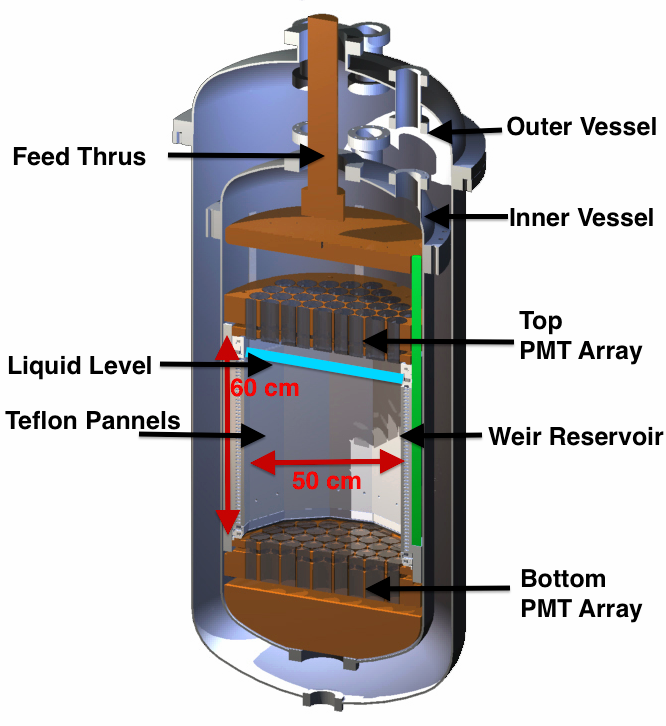
\includegraphics[scale=0.5]{Chapter_LUX_Det/LUX_half_rendering_white_text.png}
\caption{Illustration of the LUX detector's internals. The detector contains two arrays of PMTs on the top and bottom housing 61 PMTs each. Teflon panels on the edges of the active region are used to reflect scintillation signals. The vertical distance between the two PMT arrays is 60 cm, and the diameter to the inner edge of the teflon panels is 50 cm. }
\label{fig:LUX_TPC}
\end{figure}

Figures \ref{fig:LUX_Real} %and \ref{fig:LUX_Davis} 
shows the LUX detector held in place by a stainless steel frame and the water tank that surrounds it. The water tank provides shielding from gammas and neutrons emanating from the surrounding rock. The water tank PMTs, may be used as an active muon veto, are also pictured along the sides of the water tank. Figure \ref{fig:LUX_TPC} show a cross sector of the LUX detector's inner and outer vessel. The LUX detector is a two phase xenon time projection chamber (TPC)  \cite{LUX_PRL}.  The detector contains two PMT arrays on the top and bottom with 61 PMTs each for a total of 122 PMTs. The quantum efficiencies range from 30 to 40\%. 

The active region consists of a 49 cm length between the cathode and gate grid with a 47 cm diameter of the dodecagonal geometry. The drift field between the cathode and gate is 170 V/cm resulting in an electron drift velocity of 1.51 mm/$\rm \mu s$. The liquid level terminates 5-6mm above the gate grid. The liquid level is precisely maintained by a weir reservoir into which xenon between the anode and gate spills. The anode grid is 1.0 cm above the gate grid and creates an extraction field of 6 [kV/cm] where electrons are removed from the liquid and accelerated causing electroluminescence in the gas phase.  LUX contains a gross mass of 370 kg of xenon of which 250 kg are in the active region.  
% 118 kg fiducial... need to explain the fiducial region

\subsection{Target Xenon}
The target xenon is commercially-available natural xenon with standard isotopic abundances (table \ref{table:Xe_Isotopes}), initially distilled to $\sim$ 1 part per million (ppm) residual air contamination ($\rm N_2$, $\rm O_2$, Ar). The commercially available xenon also contained $\sim$ 100 parts per billion (ppb) of krypton which is far greater than the background allowance of 5 parts per trillion (ppt). Krypton contains trace amounts of a beta emitter $\rm ^{85}Kr$ and is a troublesome internal background dissolved uniformly directly in the detection medium (xenon). The unwanted krypton was removed from the bulk xenon using a gas chromatography technique \cite{lux_kr_removal}, with the removal independently verified before the science run with a xenon gas analysis technique developed for EXO-200 and LUX \cite{Kr_ppt_Dobi}. The xenon purity was monitored daily throughout the 2013 science run by an in situ gas analysis system which will be described in a future LUX publication. Just one standard liter of air contains enough krypton to raise the concentration in the LUX xenon above the background goals. Daily krypton monitoring ensured that the krypton content in the xenon remained constant at 4 parts per trillion over the 2013 science run\cite{LUX_BG}.


Electronegative impurities such as $\rm N_2$, $\rm O_2$ and $\rm H_2O$ attenuate electrons drifting through the xenon and must be removed in order to properly reconstruct events originating deep in the detector. These impurities continuously emanate from detector components degrading the free electron attenuation length. The accumulation of electronegative impurities is countered by circulating the xenon at 26.5 SLPM through a heated zirconium getter. The gross mass of 370 kg has a turn over time of 1.65 days. Throughout the 2013 science the electron attenuation length was measured to be 75 cm to 150 cm, corresponding to 70\% to 50\% charge loss for events originating from the bottom of the active region.

\renewcommand{\baselinestretch}{1}
\small\normalsize
\begin{table}[h!]
%\footnotesize
\begin{center}
\begin{tabular}{|c|c|}
\hline
Isotope & Natural \\
		& Abundance (\%) \\ \hline
$\rm^{124}Xe$ & 0.09 \\ \hline
$\rm^{126}Xe$ & 0.09 \\ \hline
$\rm^{128}Xe$ & 1.92 \\ \hline
$\rm^{129}Xe$ & 26.44 \\ \hline
$\rm^{130}Xe$ & 4.08 \\ \hline
$\rm^{131}Xe$ & 21.18 \\ \hline
$\rm^{132}Xe$ & 26.86 \\ \hline
$\rm^{134}Xe$ & 10.44 \\ \hline
$\rm^{136}Xe$ & 8.87 \\ \hline
\end{tabular}
\caption{Xenon isotopic abundances, from \cite{Xe_Isotopes}}
\label{table:Xe_Isotopes}
\end{center}
\end{table}
\renewcommand{\baselinestretch}{2}
\small\normalsize


\subsection{Background Rejection}
\label{sec:BG_Rejection}
Liquid xenon at 178 K has a density of $\sim$ 2.88 g/cm, providing excellent stopping power for shielding against external radioactivity. External radioactivity with energies in the WIMP search region of interest (below 50 keV) only penetrate millimeters in liquid xenon, being completely absorbed in the outer edges of the detector. Gammas in the MeV range have mean free paths on the order of 3 cm and are likely to be rejected by the single scattering requirement . The most troublesome of the gamma backgrounds are from PMT materials containing trace amounts of uranium and thorium located inside the TPC. Figure \ref{fig:LUX_BG_Rejection} shows a simulation of expected gamma background events inside the LUX detector, using the single scatter cut requirement. By removing the edge events we gain at least an additional factor of 1000 background rejection within the fiducial volume (inside the black dashed lines) \cite{LUX_BG}.

 \begin{figure}[h!]\centering
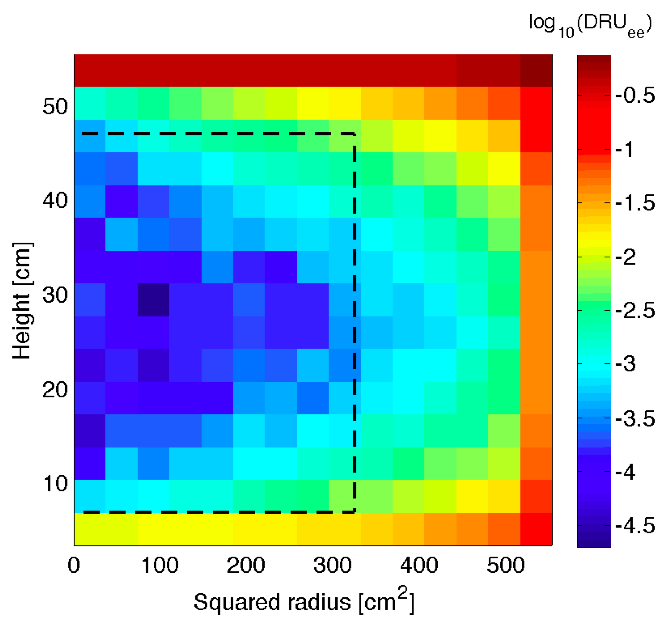
\includegraphics[scale=.4]{Chapter_LUX_Det/BG_Rejection.png}
\caption{Simulation of expected gamma background events inside the LUX detector, using the single scatter cut requirement\cite{LUX_BG}. There is a factor of 1000 background rejection within the fiducial volume where the WIMP search is conducted (inside the black dashed lines) .}
\label{fig:LUX_BG_Rejection}
\end{figure}

Another means for discriminating background events is through measuring the charge-to-light ratio of each event. WIMPs will produce nuclear recoils whereas gammas and betas interact primarily with atomic electrons, resulting in different charge to light ratios of a given energy deposit. Using $\rm AmBe$ and $\rm ^{252}Cf$ neutron sources along with a tritium calibration source, the NR to ER discrimination factor was measured to be 99.6$\pm$1 \% at 50\% NR acceptance (in section \ref{sec:ER_Discrim}). This means that only one in 250 of the residual gamma and beta background events is expected to fake a WIMP signal when cutting out half of the potential nuclear recoil candidates. The ER type and NR type bands are shown in figure \ref{fig:LUX_ER_NR_Band} with the band means as solid lines (Blue and Red, respectively) and the 10-90\% CL as dashed lines. The internal tritium calibration source will be discussed in chapter \ref{Ch:T}.

 \begin{figure}[h!]\centering
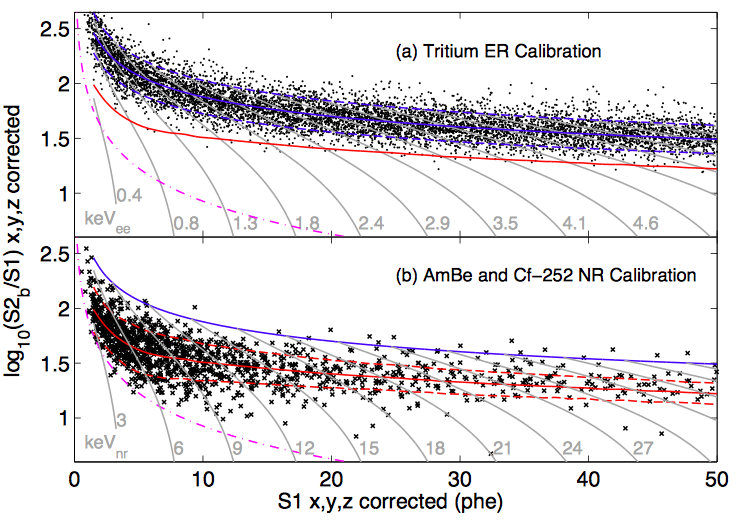
\includegraphics[scale=.5]{Chapter_LUX_Det/ER_NR_Band_Cal.png}
\caption{Plot of the log of the charge-to-light ratio vs. S1 (energy). The variable $\rm log_{10}(S2_b/S1)$ is used to distinguish ER type events from NR type events. The ER and NR bands are defined from calibrations, a) Betas from a tritium calibration (Blue), and b) Neutrons from $\rm AmBe$ and $\rm ^{252}Cf$ (Red). The band means are solid lines and the 10-90\% CL are shown as dashed lines. The ER to NR discrimination by using the charge to light ratio was measured to 99.6$\pm$0.1 \% at 50\% NR acceptance \cite{LUX_PRL}.}
\label{fig:LUX_ER_NR_Band}
\end{figure}

\newpage

\subsection{The Drift Field inside the LUX TPC}

The LUX TPC contains five wire grids used to control the electric fields inside the detector. The grids and their spacings are shown in figure \ref{fig:LUX_Fields}, labeled from top to bottom as Top  (T), Anode (A), Gate (G), Cathode (C), Bottom (B). The grids T,A,G,C,B are biased at -1,+3.5,-1.5,-10,-2 (all in kV), respectively. The PMT photocatchodes are biased to -1.2 kV on average. The field created in the active liquid xenon region between the cathode and gate is also shown in figure \ref{fig:LUX_Fields}. On average the drift field is 170 V/cm with variation from 140 V/cm to 200 V/cm  from cathode to gate. The extraction region between the anode and gate has a 6 kV/cm field. This extraction field is used to create the secondary scintillation (S2) signal via electroluminescence as the electrons are extracted and accelerated. The top and bottom grids serve to shield the PMTs from the anode and cathode voltages.  

 \begin{figure}[h!]\centering
%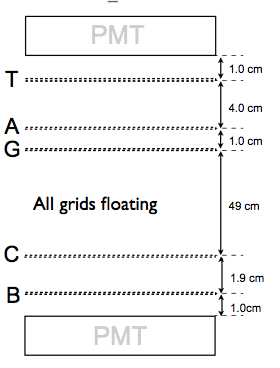
\includegraphics[scale=.75]{Chapter_LUX_Det/LUX_Feild_Grids.png}
%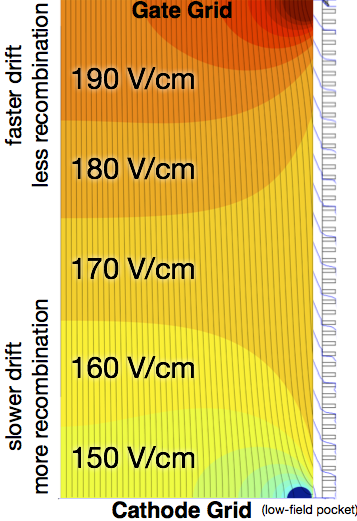
\includegraphics[scale=.56]{Chapter_LUX_Det/fieldstrength_z_vs_r.png}
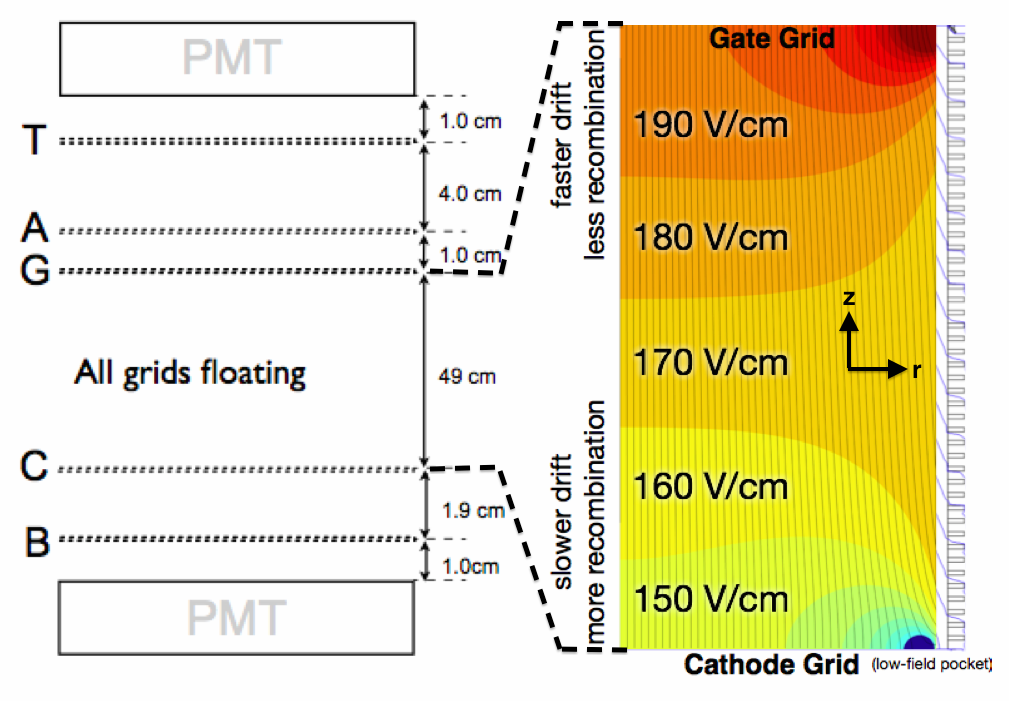
\includegraphics[scale=.4]{Chapter_LUX_Det/LUX_Feild_Grids_with_Field.png}
\caption{Field grids in the LUX detector during the 2013 science run. T,A,G,C,B are biased to -1,+3.5,-1.5,-10,-2 (all in kV), respectively. The PMTs are biased to -1.2 kV on average. The figure on the right shows the electric field model in the drift region between the cathode and gate for drift distance z vs. detector radius r. On average the drift field is 170 V/cm with variation from 140 V/cm to 200 V/cm  from cathode to gate. Electric field model from  \cite{Scott_E_Field}.}
\label{fig:LUX_Fields}
\end{figure}

\newpage

\section{Light and Charge Signals in Liquid Xenon}
\label{sec:LXe_Theory}
When energy is deposited in the active region of the xenon TPC it is converted to ionization, atomic excitation and heat.
\begin{equation}
\begin{split}
\rm E= W (n_i + n_{ex}) + Heat \\
\rm E= W \times n_q + Heat
\end{split}
\label{eq:E_Q}
\end{equation}

\noindent where E is the energy of the deposition in keV,  $\rm n_i$, $\rm n_{ex}$ and $\rm n_q$ are the number of ions, excitons and quanta respectively. An exciton is a bound state of an electron the xenon ion. The work function (W) for xenon has been measured to be 13.7 $\rm \pm$ 0.2  eV/quanta  \cite{Dahl_Thesis}. 

The number of photons produced in an event is equal to number of  initial excitons in addition to the excitons resulting from ions which recombine with freed electrons. Each de-excitation of an exciton produces one photon. The number of electrons produced in an event is equal to the number of electron-ion pairs which do not recombine.

\begin{equation}
\begin{split}
\rm  n_\gamma = n_{ex} + n_i r = n_i (r+\alpha) \\
\rm  n_e = n_i (1-r)
%\rm r= \frac{\frac{n_\gamma}{n_e}-\alpha}{\frac{n_\gamma}{n_e} + 1} %recombination fraction... mention later in detail
\label{eq:Quanta_Production}
\end{split}
\end{equation}

\noindent where $\rm n_\gamma$ and $\rm n_e$ are the number of photons and electrons and quanta. The value of r is the electron-ion recombination probability and $\rm \alpha$ represents the ratio $\rm n_{ex}/n_{ion}$. Note, $\rm n_{ex}$ represents the number of primary excitons. The model given in equation \ref{eq:Quanta_Production} states that for each additional photon produced from recombination a corresponding electron is lost, and visa versa. The value of $\rm \alpha$ for an ER event is approximately 0.2 and is expected to be independent of energy \cite{Doke_alpha} \cite{alpha_argon}. For nuclear recoils $\rm \alpha$ is approximately 1 \cite{Dahl_Thesis}. Equation \ref{eq:Q} can be written in terms of the number of photons and electrons for each energy deposit \cite{Platzman}.

\begin{equation}
\rm E= W (n_\gamma + n_e) + Heat \\
\label{eq:E_Q2}
\end{equation}

\noindent The light and charge production in liquid xenon will be discussed in further detail below. Some useful properties of xenon are listed in table listed in table \ref{table:Xe_Properties}. 

%table with Xe properties 
\renewcommand{\baselinestretch}{1}
\small\normalsize
\begin{table}[h!]
%\footnotesize
\begin{center}
\begin{tabular}{|c|c|c|}
\hline
Parameter & Value & Ref.\\ \hline
Scintillation wavelength		& 174-178 nm 		&  \cite{Doke_Scintillation} \\ \hline
W (work function)				& 13.7$\pm$0.2 [eV/quanta]	&  \cite{Dahl_Thesis} \\ \hline
$\rm Xe^*_2$	singlet lifetime	& 3.1$\pm$0.7 ns			& \cite{Xe_singlet_tripplet_lifetime} \cite{Xe_Recombination_Time}  \cite{Mock}\\ \hline
$\rm Xe^*_2 $ triplet lifetime 	& 24$\pm$1 ns			&  \cite{Xe_singlet_tripplet_lifetime} \cite{Xe_Recombination_Time}  \cite{Mock}\\ \hline
Recombination time 			& 7.5 ns $^{**}$			 & \cite{Recomb_Time_Extraction} \cite{Mock}\\ \hline
Liquid density at boiling point	& 2.95 g/l 					& \cite{Xe_Density} \\ \hline
\end{tabular}
\caption{Properties of xenon. $^{**}$ The expected recombination for the LUX drift filed of 170 V/cm. Recombination time ranges from 0 to 46 ns depending on electric field, energy deposit, and interaction type \cite{Mock} \cite{Recomb_Time_Extraction}.}
\label{table:Xe_Properties}
\end{center}
\end{table}
\renewcommand{\baselinestretch}{2}
\small\normalsize


\subsection{Electronic Recoils (ER)}
For an electronic recoil event the energy lost to heat is only about 5\% \cite{FanoTheoretical} thus, equation \ref{eq:E_Q} is valid for use with electronic recoils, we simply drop the small loss to heat. A schematic of an ER event is shown in figure \ref{fig:TomS_ER} which we describe here.

\renewcommand{\baselinestretch}{1}
\small\normalsize
\begin{figure}[h!]\centering
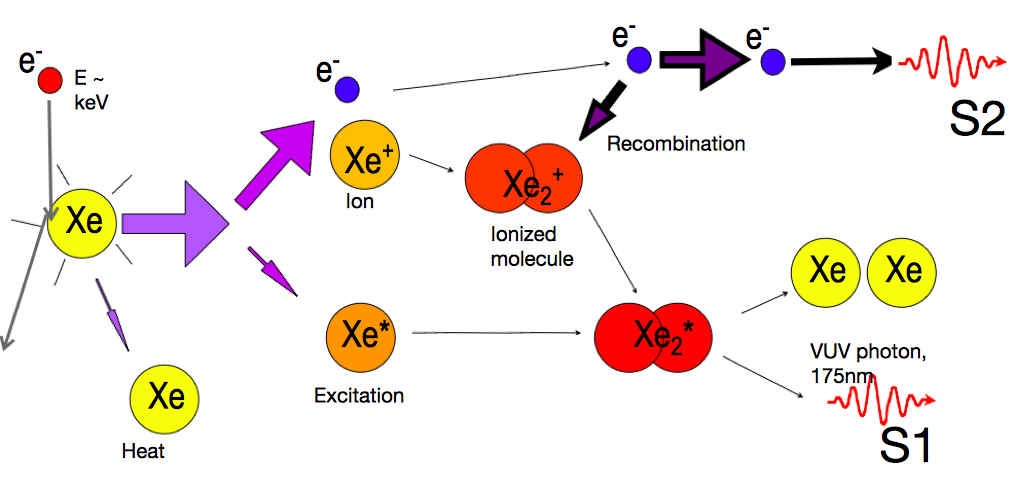
\includegraphics[width=130mm]{Chapter_LUX_Det/ER_T_Shutt.png}
\caption{An electronic recoil (ER) event in xenon. The energy deposited is converted primarily to ionization and roughly one tenth for excitation. Only several percent is lost to heat. Xenon excitons and recombining electron ion pairs from xenon dimers which de-excite producing vacuum ultra-violet  (VUV) scintillation light at 175 nm producing the primary scintillation signal (S1). Electrons that do not recombine are drifted by an electric field into the gas phase where they are accelerated producing the secondary scintillation (S2) signal. Figure from \cite{T_Shutt}.}
\label{fig:TomS_ER}
\end{figure}
\renewcommand{\baselinestretch}{2}
\small\normalsize


\noindent When an incoming beta or gamma interacts with the electron of the xenon atom, the energy deposited is converted primarily to ionization,  with roughly 6\% excitation and $\sim$ 5\% is lost to heat \cite{alpha_xenon} \cite{FanoTheoretical}. Excitons arise from ionized xenon atoms that bond together forming diatomic molecules ($\rm Xe^*_2$). Xenon excitons will de-excite with characteristic time constants of 2.2 and 27 ns for the singlet and triplet state, respectively, producing $\sim$175 nm scintillation light. Ion-electron pairs produced via ionization can also recombine, with probability r, producing additional excitons resulting in the production of additional $\sim$175nm scintillation light. The characteristic recombination time constant in LUX is 7.5 ns \cite{Xe_Recombination_Time}. Each initial exciton or recombining ion produces one scintillation photon, as written in equation \ref{eq:Quanta_Production}. The two paths for photon production overlap in time and sum to produce the primary scintillation signal (S1). %In LUX the S1 signal is collected by the PMT arrays within 50 ns. 

Electrons that escape recombination, with probability 1-r, begin to drift upwards under the influence of the electric field between the cathode and gate (shown in \ref{fig:LUX_Fields}). The electrons eventually reach the liquid-gas interface where they are extracted into the gas. As they accelerate, the extracted electrons produce a larger secondary scintillation signal (S2) that is proportional the the number of electrons extracted. The drift times for the electrons in the 49 cm, vertical length, active region range from 1 to 324 $\rm \mu s$ with an average drift velocity of 1.51 mm/$\rm \mu s$. Thus, the S2 signal is well separated from the S1. 


\subsection{Nuclear Recoils (NR)}
For nuclear recoils the energy lost to heat is more than half the total energy deposition \cite{FanoTheoretical}. This energy is lost through elastic collisions with other xenon atoms that fall below the ionization threshold. The energy lost to heat is characterized by an energy dependent Lindhard factor ($\mathcal{L}$) \cite{Lindhard}, written as: 

\begin{equation}
\rm E=\mathcal{L}^{-1}W (n_\gamma + n_e)
\label{eq:Lindhard}
\end{equation}

A schematic of a NR event is shown in figures figure \ref{fig:TomS_NR}. The signal production follows the same process as described above for an ER event but with greater amount of energy going towards heat and exciton production. 

\renewcommand{\baselinestretch}{1}
\small\normalsize
 \begin{figure}[h!]\centering
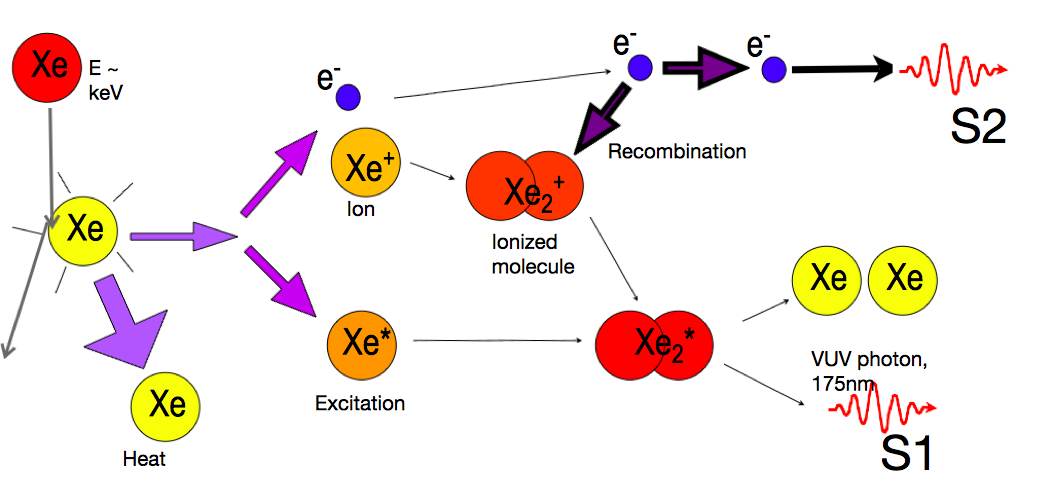
\includegraphics[width=130mm]{Chapter_LUX_Det/NR_T_Shutt.png}
\caption{A nuclear recoil (NR) event in xenon. The energy deposited goes mainly towards heat (phonons), the remaining energy is split evenly between ionization and excitation. Xenon excitons and recombining electron ion pairs for xenon dimers which de-excite producing vacuum ultra-violet  (VUV) scintillation light at 175 nm producing the primary scintillation signal (S1). Electrons that do not recombine are drifted in an electric field into the gas phase where they are accelerated producing the secondary scintillation (S2) signal. Figure from \cite{T_Shutt}. }
\label{fig:TomS_NR}
\end{figure}
\renewcommand{\baselinestretch}{2}
\small\normalsize

\noindent The additional energy lost to heat leaves less energy available for excitation and ionization for an NR event. Further, NR events produce roughly equal amounts of ionization and excitation whereas ER events produce mostly ionization \cite{FanoTheoretical}  \cite{Dahl_Thesis}. Relative to an ER event, a NR event will have less electron ion pairs leading to a reduction of the S2 signal and enhancement the S1. Thus, the ratio of S2 to S1 for a NR event is ``quenched", or smaller, compared to an ER event with an equivalent energy deposition. The quenching of the charge to light ratio is what allows for discrimination between nuclear and electronic recoils as demonstrated in figure \ref{fig:LUX_ER_NR_Band}.

\subsection{Energy and Position Reconstruction}
In order to reconstruct the true energy of an event we need to know its nature, ER or NR. For ER events we work in units of electronic equivalent energy, ($\rm keV_{ee})$, using equation \ref{eq:E_Q} and neglecting the small heat loss. ER calibrations will be discussed in greater detail in chapter \ref{Ch:E_Scale_Cal}. For NR events the energy is reconstructed in terms of nuclear recoil equivalent energy ($\rm keV_{nr}$), using equation \ref{eq:Lindhard} with the Lindhard factor measured from calibration data given in \cite{NEST} \cite{NEST_2013}.  

An illustration of an energy deposition in the LUX detector is show in figure \ref{fig:LUX_Event}. The time difference between the S1 and S2 pulse defines the drift time, the drift time gives the measure of the z coordinate (depth). The hit pattern of the S2 signal on the top PMT array measures the x,y coordinates of the event. From the S1 and S2 signals the full x,y,z position and the energy of the event can be reconstructed.

 \begin{figure}[h!]\centering
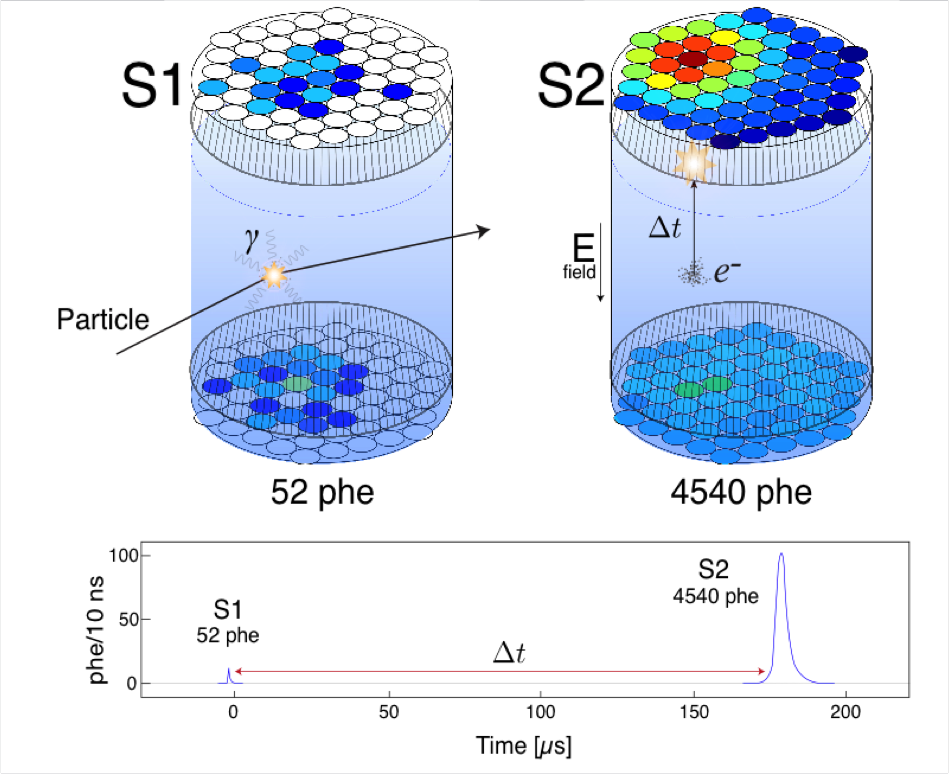
\includegraphics[width=150mm]{Chapter_LUX_Det/LUX_Event_Diagram.png}
\caption{Event diagram.}
\label{fig:LUX_Event}
\end{figure}

\section{Identifying S1, S2}
The primary and secondary scintillation signals can be identified by their unique properties. The S1 signal has a fast rise time and decays on the order of 10's of nano-seconds as the dimers of xenon produced through excitation and recombination de-excite (time constants listed in table \ref{table:Xe_Properties}). The S2 signal arrives several $\rm \mu s$ later with the electron population spread out spatially about its centroid due to diffusion, transverse and radial \cite{Electron_Diffusion}. The characteristic S2 signal is thus one with a slow rise and corresponding slow fall. It resembles a bell curve, as the diffused electron population arrives, peaking at the centroid of the distribution. A 2 keV event as seen by all 122 PMT channels is shown in figure \ref{fig:LUX_Golden}. The S1 pulse is fast and the S2 pulse is much larger with a slower rise-time.  The S2 pulse is larger since a single electron creates hundred of photons as it is accelerated in the extraction region. 

%Show prompt fraction plot to describe event selection.

 \begin{figure}[h!]\centering
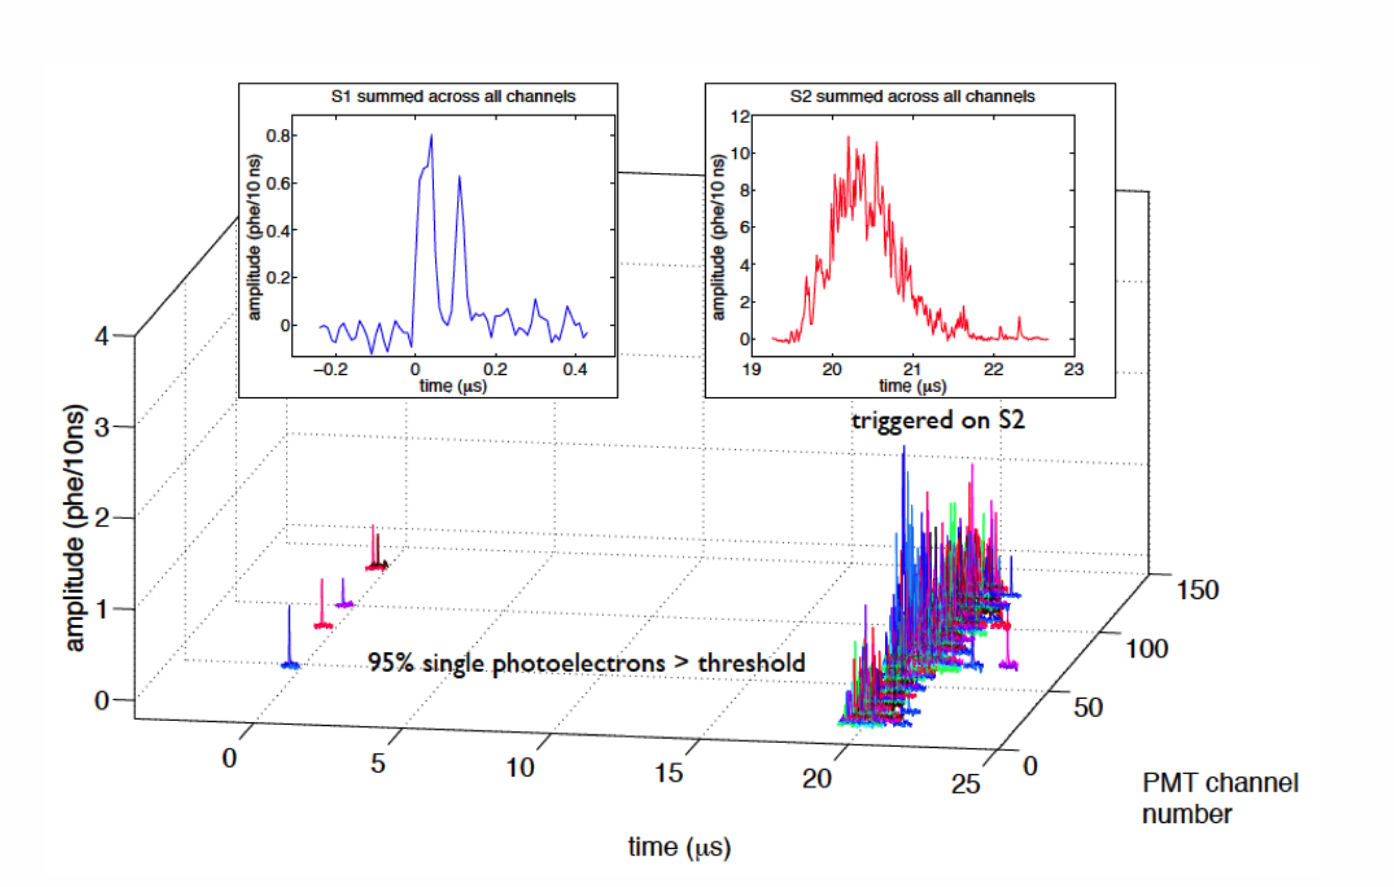
\includegraphics[width=130mm]{Chapter_LUX_Det/LUX_Golden_Event_2keV.png}
\caption{ 2 keV ER event as seen by each PMT channel of the LUX detector. The S1 signal summed across all channels is overlaid on the top left, and the S2 signal summed across all channels is overlaid on the top right.}
\label{fig:LUX_Golden}
\end{figure}

To identify S1 and S2 populations we define the variable ``Prompt Fraction" as the area covered in the first 10\% of the pulse waveform normalized to the total area. The calculation is performed on the summed waveform after a first pass which defines the pulse's start and end timestamp. 
%For S1s this value will approach 1 and for S2s the value will be below 0.1, this provides for a figure of merit used to separation of the populations.
The separation of population density when plotting the total Pulse Area (measured in detected photo electrons [PE]) vs. Prompt Fraction is shown in figure \ref{fig:Prompt_Fraction},  for the case of a $\rm ^{83m}Kr$ data set (41.5 keV) and a tritium calibration data set (1-18.5 keV). The population of single electrons, single photons and the S1 S2 pairs associated with $\rm \gamma$, $\rm \beta$ and $\rm \alpha$ interactions are well separated and are highlighted as rectangles. The upper left corner is the single photon population. The area is approximately 1 PE, this defines the PMTs' response to a detected photon. The single electron population is labeled SE and peaks at roughly 20 PE with a prompt fraction of 0.1. For all S1 pulses the prompt fraction is found to be between 1 and 0.3 ($\rm log_{10}$ of 0 and -0.5) for the entire range of Pulse Area. The pulse area is a proxy for energy, spanning from 1 keV tritium events to 7 MeV alphas. The populations of S2 from $\rm^{83m}Kr$, tritium, $\rm \gamma$, $\rm \beta$ and $\rm \alpha$ are found to have Prompt Fractions more than an order of magnitude smaller than their corresponding S1. 
%Note: The double population seen in the $\rm^{83m}Kr$ S1 population is the result of double decay separated by 154 ns which can skew the apparent prompt fraction to lower values, discussed further in [XYZ Corrections].


The S1 and S2 signals corresponding to an event are identified using a prompt fraction selection that has been tuned to calibration data. Valid S1 and S2 signals that spill into the single electron and single photon region at low energies can be identified by requiring the pulses be paired. For the WIMP search we define `golden' events consisting of single scatters with a single S1 paired with a subsequent S2 pulse with a timing separation within the maximum drift time of the TPC. With the golden requirement each event has a well defined x,y coordinate and z making it possible to correct the signals for geometrical effects and electron attenuation. 

 \begin{figure}[h!]\centering
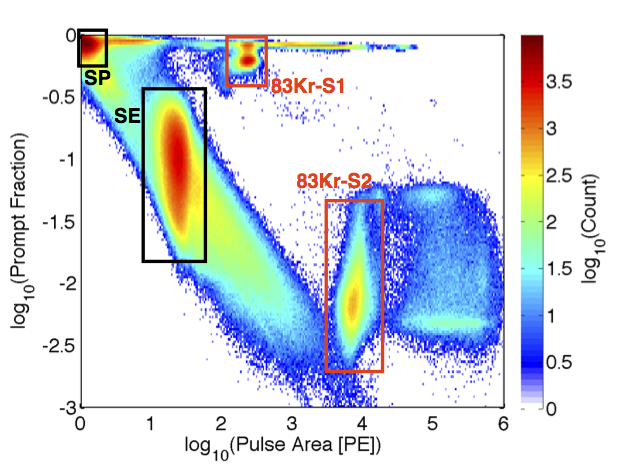
\includegraphics[width=110mm]{Chapter_LUX_Det/Kr_83_Density_text.png}
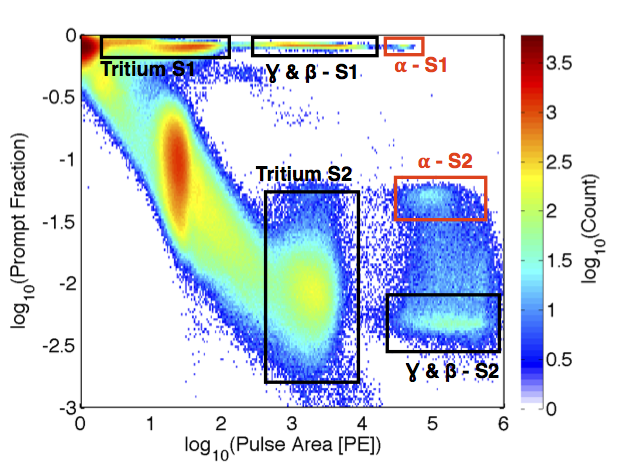
\includegraphics[width=110mm]{Chapter_LUX_Det/T_Density_text.png}
\caption{Density plot of prompt fraction vs. Pulse Area. Top: $\rm^{83m}Kr$ data set. Bottom: Tritium data set. Populations of single electrons, single photons and the S1 S2 pairs associated with $\rm \gamma$, $\rm \beta$ and $\rm \alpha$ are highlighted as rectangles.}
\label{fig:Prompt_Fraction}
\end{figure}


\section{LUX Science Result (WIMP limit)}

The first science run of the LUX detector consisted of 85.3 live days between April 21, 2013 to Aug 8, 2013. A total of 83,673,413 triggers were recorded with 160 remaining as golden after applying quality cuts, listed in table \ref{table:WIMP_Quality_Cuts}.  

\renewcommand{\baselinestretch}{1}
\small\normalsize
\begin{table}[h!]
%\footnotesize
\begin{center}
\begin{tabular}{|c|c|}
\hline
Cut & Events Remaining \\ \hline
all triggers & 83, 673, 413 \\ \hline
detector stability & 82, 918, 902 \\ \hline
single scatter & 6, 585, 686 \\ \hline
S1 energy (2 - 30 phe) & 26, 824 \\ \hline
S2 energy (200 - 3300 phe) &  20, 989 \\ \hline
single electron background & 19, 796 \\ \hline
fiducial volume & 160 \\ \hline
\end{tabular}
\caption{Data quality cuts used for the WIMP search results presented in \cite{LUX_PRL}.}
\label{table:WIMP_Quality_Cuts}
\end{center}
\end{table}
\renewcommand{\baselinestretch}{2}
\small\normalsize

\noindent Detector stability cuts remove the live time in which liquid level, gas pressure or grid voltages were out of normal ranges. The single scatter cut requires a single S1 with a subsequent S2 within a time window of 324 $\rm \mu s$, the maximum time required for electrons to traverse the active region. An area cut was also placed on both the S1 and S2 in order to narrow the energy region of interest. The minimum S2 requirement of 200 PE ensures the quality of the x,y position reconstruction, with $\sim$ 8 extracted electrons. An additional cut was placed around time windows with anomalously high single electron rates. All single scatter WIMP search events before applying the fiducial cut are shown in figure \ref{fig:LUX_Result_Event}, the vast majority of events occurring at the edges of the detector. 
The fiducial cut reduces residual radioactivity from the detector surface and PMTs by another two orders of magnitude. The fiducial cut consists of a radial cut at radius less than 18 cm from the detector center. The z coordinate in drift time is defined to be 0 $\rm \mu s$ at the liquid surface and 324 $\rm \mu s$ at the cathode. The fiducial cut in z required that event drift times be between 38 and 305 $\rm \mu s$, corresponding to 6 to 46 cm below the liquid surface (drift velocity = 1.51 mm/$\rm \mu s$). The fiducial cut is shown as the dashed cyan line in figure \ref{fig:LUX_Result_Event}.

 \begin{figure}[h!]\centering
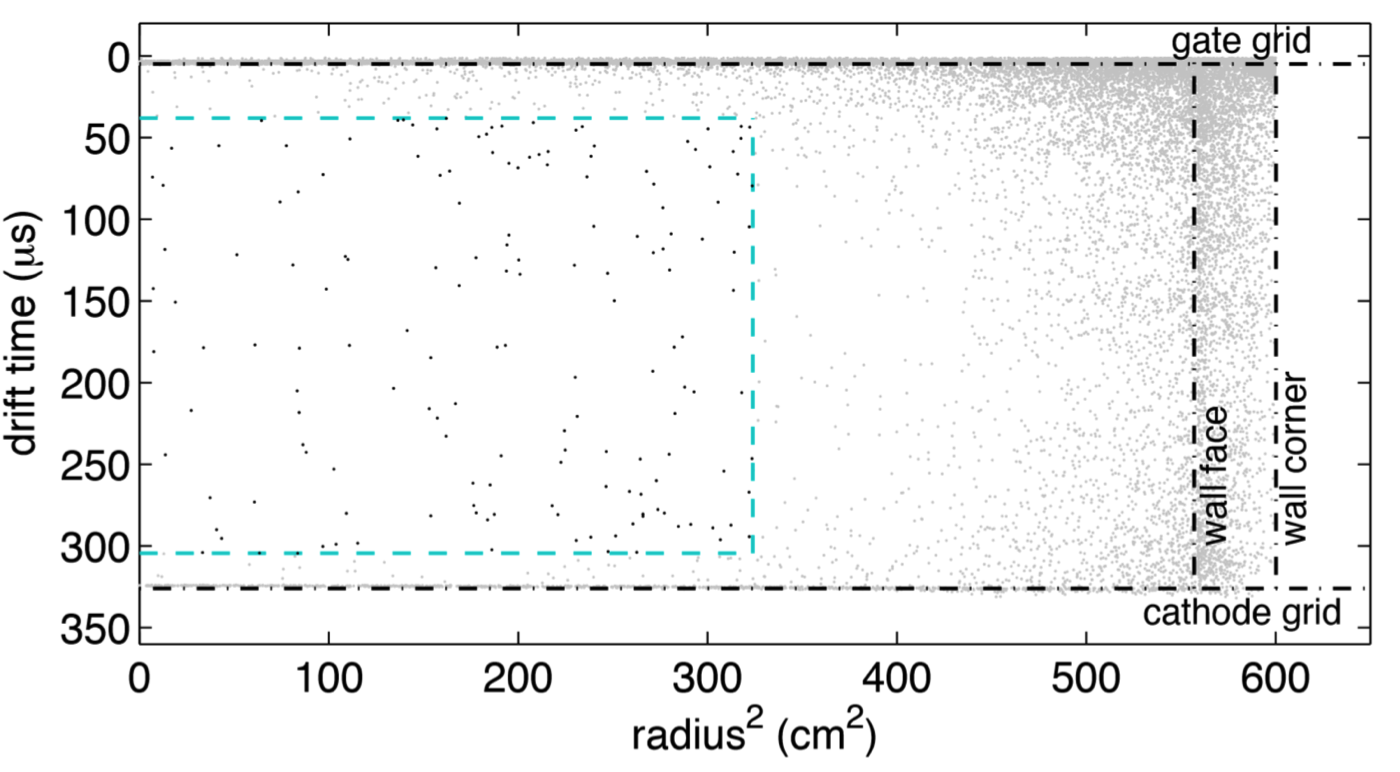
\includegraphics[width=130mm]{Chapter_LUX_Det/LUX_Result_Event.png}
\caption{All single scatter events seen in the active region of the LUX detector over the course of the first science run passing all cuts listed in table \ref{table:WIMP_Quality_Cuts} excluding the fiducial cut. The dashed cyan box indicates the fiducial volume.}
\label{fig:LUX_Result_Event}
\end{figure}

Within the fiducial volume 160 events remain which meet our WIMP search energy requirement. The energy cut is placed in terms of S1 from 2-30 PE. As explained in chapter \ref{Ch:E_Scale_Cal}, this corresponds to roughly 1.0 to 6 $\rm keV_{ee}$ or 3 to 25 $\rm keV_{nr}$. We choose to select events based on S1 because it is directly observed, whereas true energy depends on the nature of the event (ER or NR) and must be inferred. %These subtletie will be discussed in further detail in this thesis. 
The ER and NR discrimination band was measured using calibration data as shown in figure \ref{fig:LUX_ER_NR_Band} is reproduced in \ref{fig:LUX_Result}. The blue and red bands represent the 10\% to 90\% confidence bounds of events being ER and NR type, respectively. The ER band was measured using a tritium calibration source ($\rm \beta^{-}$) and the NR band was measured with neutrons from AmBe and $\rm^{252}Cf$ along with NEST simulations \cite{NEST_2013}. The ER/NR discrimination at 50\% NR acceptance was measured to be $\rm 99.6\pm0.1$ \%. This value serves as a measure of background rejection, which is ultimately treated with a profile likelihood method on an event-by-event basis. Both the S1 and S2 signal have been corrected for spatial dependance, as discussed in further detail in Chapter \ref{Ch:3}. %Due to cross talk or shorts, two PMTs on the top array and one on the bottom were left unbiassed.  In order to avoid misreconstructing events extracted around the unbiased top PMTs only the bottom PMT array was used for the S2 signal ($\rm S2_b$).

 \begin{figure}[h!]\centering
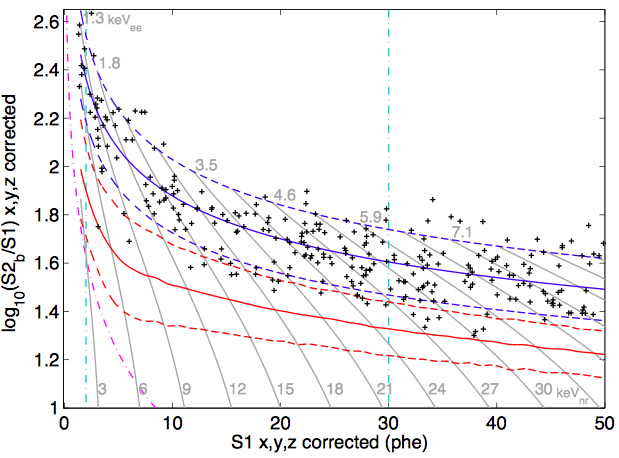
\includegraphics[width=120mm]{Chapter_LUX_Det/LUX_Result.png}
\caption{The remaining events passing the quality cuts listed in table \ref{table:WIMP_Quality_Cuts}. The charge to light ratio (S2/S1) is plotted vs. S1 (proportional to energy) to show the separation of ER and NR type events. The 10-90\% CF limits of the ER and NR band are plotted as the dashed blue and red curves, respectively. The band means are solid. $\rm S2_b$ stands for the S2 signal on the bottom PMT array. }
\label{fig:LUX_Result}
\end{figure}

\newpage

All 160 remaining events in the fiducial volume are consistent with being ER type events. The main source of background events include residual $\rm^{85}Kr$, activated $\rm^{127}Xe$ and $\rm^{214}Pb$ from $\rm^{222}Rn$, described in further detail in \cite{LUX_BG}. The residual ER background rate in the WIMP region of interest as found to be 3.6$\rm\pm$0.3 mDRU ($\rm 10^{-3}$ cnts/keVee/kg/day) with an expectation of 2.6$\rm\pm 0.2_{stat}$ $\rm\pm 0.4_{sys}$ mDRU.


A profile likelihood test is conducted on all WIMP search candidates remaining after the cuts listed in table \ref{table:WIMP_Quality_Cuts}. The signal model is derived from AmBe and $\rm^{252}Cf$ neutron calibrations. The background rates input into the profile likelihood were independently measured and modeled with LUXSIM using NEST, described in further detail in \cite{LUX_BG} \cite{LUX_PRL} \cite{NEST_2013}. The WIMP signal model was generated using an isothermal halo with a Maxwellian distribution, with a local WIMP density of 0.3 GeV/$\rm cm^3$ (as discussed in section \ref{sec:DM_Search}). The galactic escape velocity input into the model is 544 km/s (cutting off the high end of WIMP velocity distribution), with an average WIMP velocity of 220 km/s. The earth's seasonal velocity being 245 km/s with respect to the galactic center. The result from the 2013 science run with the LUX detector is consistent with a P value of 0.35 for the background-only hypothesis. The 90\% upper C.L. cross section for various spin independent masses are shown in figure \ref{fig:LUX_Limit}. The minimum cross section reported occurs at 7.6$\rm\times10^{-46}$ $\rm cm^2$ for a WIMP mass of 33 GeV/$\rm c^2$ \cite{LUX_PRL}. The LUX result is a factor of two improvement in WIMP cross section sensitivity over the Xenon100 limit reported in 2012 \cite{Xenon100} and is in tension with reported WIMP signal claims from CoGent \cite{CoGeNT}, CDMSLite (Silicon) \cite{CDMSlite}, CRESST II \cite{CRESSTII} and DAMA/LIBRA \cite{DAMA}.

 \begin{figure}[h!]\centering
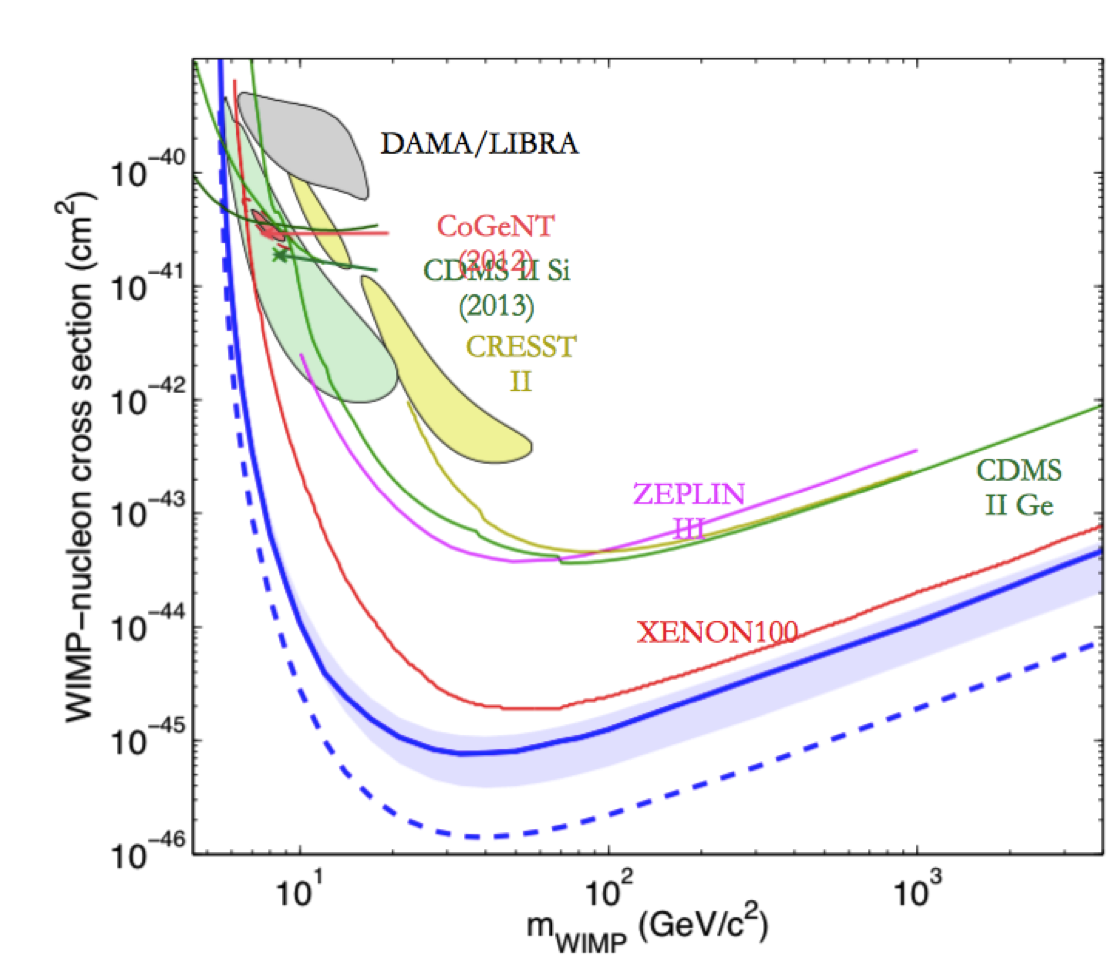
\includegraphics[width=120mm]{Chapter_LUX_Det/LUX_Limit.png}
\caption{LUX detector is consistent with a P value of 0.35 of the background only hypothesis. The 90\% upper C.L. cross section for various spin independent masses are shown in figure \ref{fig:LUX_Limit} in blue. Also shows are limits from Xenon100 (red), CDMS II (green), ZEPLIN III (magenta), and one sigma signal claimed for DAMA/LIBRA (shaded grey), CDMS II Silicon (shaded green), CRESST II (shaded yellow).}
\label{fig:LUX_Limit}
\end{figure}

\newpage

As mentioned above the ER band is measured with a tritium calibration source and will be discussed in further detail in chapter \ref{Ch:T}. Since the initial science run we have gathered twenty times the tritium statistics to further study the ER band, with over 140,000 tritium events in the fiducial volume. We also spent several months calibrating the LUX detector with a DD neutron generator to further study the NR band mean. The results from the improved ER calibrations will be reported here and will be used for a reanalysis of the LUX WIMP search data. The result will be submitted for publication in late 2014. 
